\documentclass[12pt]{report} 

% language may be romanian or english (default is english)
% type may be bachelor or master (default is bachelor)
\usepackage[language=english, type=bachelor]{style}

\usepackage{fancyhdr}
\pagestyle{fancy}
\lhead{}
\chead{}
\renewcommand{\headrulewidth}{0.2pt}
\renewcommand{\footrulewidth}{0.2pt}

\begin{document}

\specialization{Computer Science}	
\title{AI-Assisted Dental Imaging Web Platform \\ \large for Automated Finding Detection}					   
\author{Alexandra Petrea}											
\supervisor{Prof. Conf. univ. dr. Christian SACAREA}				
				
\maketitle

\newpage
\thispagestyle{empty}
\mbox{}
\newpage
\pagenumbering{roman} 

\cleardoublepage
ABSTRACT
\vspace{0.5cm}	
\hrule
\vspace{0.5cm}	

This bachelor thesis presents the development of an AI-assisted web platform designed to automate the detection of dental anomalies using the Faster R-CNN object detection architecture. By training on a comprehensive dataset of panoramic and bitewing radiographs, the proposed system aims to demonstrate high precision in localizing interproximal caries, impacted teeth, and periapical lesions. The research bridges the gap between deep learning technologies and clinical diagnostics, providing a secure, user-friendly interface that serves as a robust second-opinion tool for modern dentistry. This automated approach prioritizing high accuracy over superficial speed is designed to reduce practitioner fatigue, minimize diagnostic errors, and ultimately optimize treatment workflows.

\tableofcontents

\newpage
\pagenumbering{arabic}

\chapter{Introduction}
\label{ch:intro}

\section{Context of the Research}
Integrating artificial intelligence into medical imaging, particularly through deep learning and convolutional neural networks (CNNs), represents a profound paradigm shift in modern dentistry \cite{alenezi2023artificial, bozkurt2023deep, khan2021clinical, lecun2015deep}. Over the past decade, the rapid advancement of computer vision architectures—most notably the "You Only Look Once" (YOLO) family of object detection models—has demonstrated exceptional capability in analyzing complex anatomical structures in real-time \cite{geetha2024ai, lin2014microsoft, redmon2016you}. Dental radiography, including panoramic and bitewing X-rays, provides critical diagnostic information; however, interpreting these multimodal images is often subjective and dependent on the practitioner's clinical experience \cite{chen2022comprehensive, kim2020automated, rahman2021deep}. Recent studies have highlighted the efficacy of advanced object detection algorithms, such as YOLOv8, in autonomously identifying and localizing various dental anomalies, including interproximal caries, periapical lesions, and impacted teeth \cite{devito2023advanced, hao2023innovative, lee2023detection, sharma2024early}. By bridging the gap between raw radiological data and actionable diagnostic insights, AI-assisted computer vision serves as an invaluable second-opinion tool in contemporary endodontic and restorative workflows \cite{endres2020development, hwang2019overview, mohammad2022deep, wang2022automated}.

\section{Problem Definition}
Despite the promising capabilities of deep learning in medical diagnostics, standardizing automated dental anomaly detection remains a highly complex scientific challenge \cite{haghanifar2020dental, jocher2023ultralytics, nguyen2023dental, schwendicke2020artificial}. The primary difficulty lies in the high variability of dental X-rays, where issues such as overlapping teeth structures, low image contrast, artifacts from metallic restorations, and diverse anatomical morphologies obscure subtle pathologies like early-stage caries or discrete periapical lesions \cite{lee2021challenges, orhan2020evaluation, tuzoff2019tooth}. Furthermore, existing AI models frequently struggle with class imbalance and inconsistent bounding box precise localization when trained on heterogeneous datasets from varying clinical environments \cite{pang2019libra, prados2020artificial, son2022performance}. While older generalized neural networks fall short of offering real-time, multi-class diagnostic precision without exhausting computational resources, state-of-the-art single-stage detectors need severe custom architectural optimization and properly mapped class ontologies to correctly differentiate between visually similar dental conditions \cite{tan2019efficientnet, xie2023survey}. Consequently, there is a critical need for an adapted, highly precise, and computationally efficient deep learning pipeline that can reliably operate on local clinical hardware without sacrificing diagnostic accuracy.

\section{Proposed Solution and Motivation}
This work investigates the development and implementation of an optimized, AI-assisted dental imaging web platform driven by a customized YOLOv8 object detection architecture. The primary objective is to train a robust neural network on a unified, comprehensively annotated dataset of dental radiographs to autonomously detect, classify, and visualize pathological findings with high diagnostic confidence. By integrating this advanced computer vision model into a secure and intuitive web interface, the research aims to provide a seamless, real-time diagnostic support tool for clinical environments. The motivation behind this endeavor is deeply rooted in enhancing diagnostic precision and reducing physician fatigue; by providing dentists with an instantaneous visualization of potential anomalies categorized by standardized classes, the proposed system aspires to significantly minimize human error, expedite treatment planning, and ultimately improve the overarching quality of patient care in modern dentistry.

%\input{chapters/chapter2}
\chapter{Theoretical Framework and Technologies}
\label{chap:ch3}

\par This chapter establishes the extensive theoretical and technological foundation required for the development of the AI-assisted dental imaging platform. It is systematically structured to transition from the fundamental concepts of artificial neural networks and deep learning in medical imaging to the explicit mathematical and architectural nuances of two-stage object detection models. Furthermore, a comprehensive analysis of the current state of research is provided to contextualize the work within modern scientific literature. Finally, a detailed justification of the specific tools and technologies selected to engineer the end-to-end platform is presented, encompassing the object detection pipeline, cloud-based hyper-accelerated training, and the integration of a generative AI API for automated treatment planning.

\section{Theoretical Background and Definitions}
\label{sec:ch3_theoretical_bg}

\subsection{Fundamentals of Artificial Neural Networks and Deep Learning}
\par The evolution of Artificial Intelligence (AI) has significantly transformed the landscape of medical diagnostics, providing novel instruments to augment human expertise. At the core of this transformation is machine learning (ML), a subset of AI that relies on statistical models to enable computer systems to perform complex tasks by learning patterns from data without explicit programming. Deep Learning (DL), an advanced and highly specialized branch of machine learning, employs multi-layered artificial neural networks capable of learning hierarchical and nonlinear representations of complex data architectures \cite{lecun2015deep}.
\par An Artificial Neural Network (ANN) mimics the biological neural pathways of the human brain. It is fundamentally composed of interconnected nodes, or "neurons," organized in distinct layers: an input layer, multiple hidden layers, and an output layer. In the context of deep learning, the term "deep" refers specifically to the presence of multiple hidden layers that allow the network to extract exponentially complex features from the raw input data.
\par The activation function within each neuron is critical to the network's ability to solve non-linear problems. Common activation functions include the Rectified Linear Unit (ReLU), which mitigates the vanishing gradient problem by outputting the input directly if it is positive and zero otherwise. The learning process of these networks is driven by the backpropagation algorithm. Backpropagation calculates the gradient of a loss function with respect to the network's weights, enabling optimization algorithms (such as Stochastic Gradient Descent or Adam) to iteratively update the parameters to minimize the error between the model's predictions and the actual ground truth.

\subsection{Convolutional Neural Networks (CNNs)}
\par While standard feed-forward neural networks are effective for structured numerical data, they are profoundly inefficient when processing high-dimensional data such as high-resolution medical imagery. This inefficiency arises from the massive number of parameters required to connect every pixel to every neuron, leading to computationally prohibitive models prone to severe overfitting.
\par Convolutional Neural Networks (CNNs) were introduced to resolve this limitation through localized feature extraction and weight sharing. A CNN applies a series of convolution operations, wherein a small matrix (a kernel or filter) slides across the input image, computing dot products at each spatial position. This process generates a feature map that highlights specific visual patterns, such as edges, textures, or gradients.
\par CNN architectures typically alternate between convolutional layers and pooling layers. Pooling (frequently Max Pooling) is a down-sampling operation that reduces the spatial dimensions of the feature maps, subsequently decreasing computational complexity while ensuring translation invariance. As the data passes deeper into the network, the extracted features become increasingly abstract; early layers might detect simple lines and corners, whereas deeper layers can identify complex morphological structures indicative of specific dental pathologies \cite{chen2022comprehensive}. In dentistry, the implementation of these CNN models signifies a shift toward automated, precision-based medicine \cite{alenezi2023artificial}.

\begin{figure}[htbp]
    \centering
    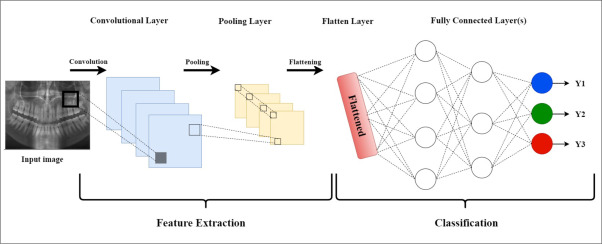
\includegraphics[width=0.8\textwidth]{figures/cnn.jpg}
    \caption{Standard block architecture and operational flow of a Convolutional Neural Network \cite{sciencedirect_cnn2026}.}
    \label{fig:cnn_arch}
\end{figure}

\subsection{Basic Principles of Object Detection in Computer Vision}
\par Object detection is a pivotal and highly challenging task in computer vision that entails two synchronous operations: identifying the presence of specific object categories within an image (classification) and delineating their exact spatial locations via bounding boxes (localization). Traditional computer vision models depended heavily on handcrafted feature extractors (such as SIFT or HOG), which lacked the robustness required for highly variable medical images. The advent of deep learning has led to an era of resilient, automated feature learning \cite{xie2023survey}.
\par Modern neural network architectures for object detection are broadly dichotomized into one-stage and two-stage detectors. One-stage detectors (e.g., YOLO variants \cite{redmon2016you}) treat object detection as a unified, single regression problem. They partition the image into a grid and simultaneously predict bounding box coordinates and class probabilities. While this single-pass architecture optimizes computational velocity and is ideal for real-time video tracking, it inherently compromises on the strict localization precision required for small objects or crowded scenes.
\par Conversely, two-stage detectors, such as the R-CNN family (including Faster R-CNN \cite{kim2020automated} and Libra R-CNN \cite{pang2019libra}), operate sequentially. The first stage generates a set of region proposals (areas of the image highly likely to contain an object), and the second stage classifies these specific regions while refining their bounding box coordinates. This rigorous methodology consistently achieves superior accuracy and handles small, difficult-to-detect objects—such as early-stage interproximal caries—exceptionally well.

\subsection{Pathological Findings in Dental Radiographs}
\par Proper comprehension of the automated detection system necessitates formal and rigorous definitions of the medical anomalies it is designed to isolate. Panoramic radiographs (orthopantomograms) and bitewing radiographs are the primary diagnostic modalities in contemporary dental practice. Due to the superimposed 3D anatomies projected onto a 2D plane, identifying minute pathologies requires substantial clinical acumen.
\par \textbf{Dental Caries:} Defined clinically as the localized destruction of susceptible dental hard tissue caused by acidic by-products from bacterial sugar fermentation. Caries detection is notoriously challenging in its incipient stages due to subtle radiographic manifestations visible only as slight radiolucencies in the enamel. High accuracy in identifying interproximal (between teeth) caries is fundamental to preventing irreversible pulp exposure \cite{schwendicke2020artificial}. In machine learning contexts, recent approaches involve consolidating heterogeneous datasets (for example, mapping distinct "Deep Caries" instances into a unified broader "Caries" class) to provide the neural network with a statistically robust number of examples, thus enhancing the generalization capabilities.

\begin{figure}[htbp]
    \centering
    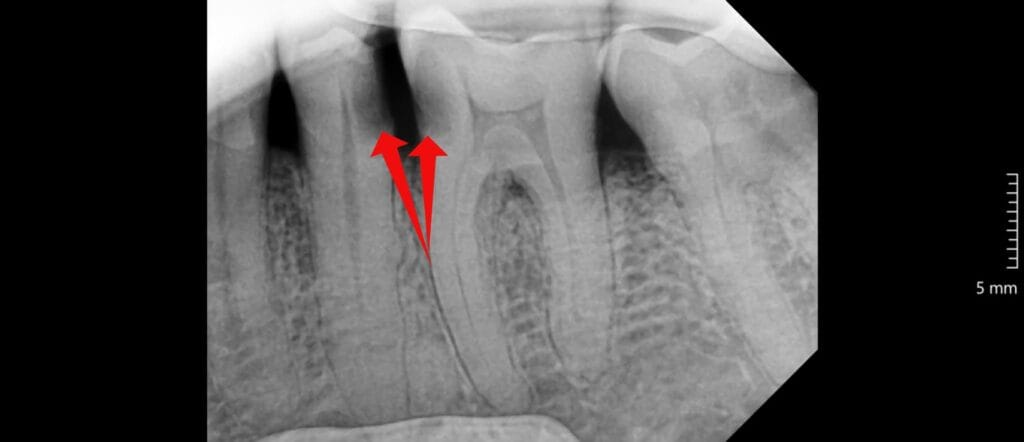
\includegraphics[width=0.6\textwidth]{figures/carie.jpg}
    \caption{Radiographic and clinical manifestation of dental caries \cite{dentalford2026}.}
    \label{fig:carie}
\end{figure}

\par \textbf{Periapical Lesions:} These are complex endodontic pathologies situated around the apex of the tooth root, manifesting predominantly as a consequence of untreated pulp necrosis. Early and accurate detection of periapical radiolucencies is highly dependent on image contrast, exposure quality, and practitioner expertise \cite{orhan2020evaluation}. Distinguishing these lesions from normal anatomical landmarks (such as the mental foramen) is a frequent point of failure for inexperienced practitioners.

\begin{figure}[htbp]
    \centering
    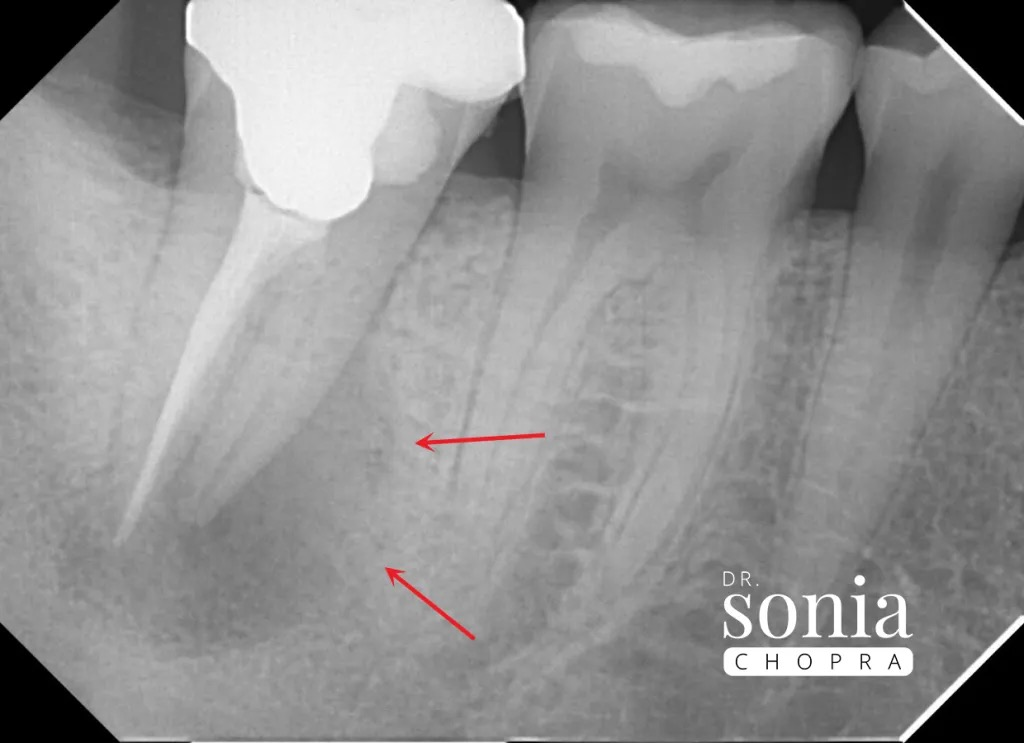
\includegraphics[width=0.6\textwidth]{figures/periapical_lesion.jpg}
    \caption{Clinical characterization and radiographic appearance of a periapical lesion \cite{chopra2026}.}
    \label{fig:periapical}
\end{figure}

\par \textbf{Impacted Teeth:} Defined as teeth that have failed to erupt fully into the functional dental arch within their expected developmental timeline constraints. Visualizing the precise angulation, root morphology, and the spatial relationship with adjacent anatomical structures (such as the inferior alveolar nerve canal) is imperative for surgical extraction planning \cite{kim2020automated}. Efficiently isolating impacted teeth as an independent diagnostic class ensures targeted reporting and avoids misclassification with normally erupting dentition.

\begin{figure}[htbp]
    \centering
    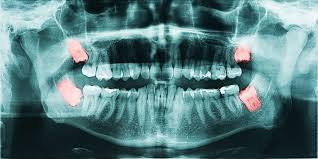
\includegraphics[width=0.6\textwidth]{figures/impacted_tooth.jpeg}
    \caption{Radiographic example of an impacted tooth obstructing adjacent structures \cite{airdrie2026}.}
    \label{fig:impacted}
\end{figure}

\section{Analysis of Current State of Research}
\label{sec:ch3_state_of_research}

\subsection{Deep Learning for Differential Diagnosis in Dentistry}
\par Research in the domain of automated dental diagnostics has gathered massive momentum, addressing the clinical necessity for objective, reproducible, and instantaneous second opinions. Hwang et al. \cite{hwang2019overview} emphasize that practitioner fatigue, cognitive bias, and varying levels of clinical experience heavily influence the interpretation of dental radiographs. Deep learning frameworks have consequently been proposed to mitigate human oversight, specifically acting to reduce the rate of false negatives (missed diagnoses) in high-throughput clinical settings.
\par The detection of dental caries remains heavily researched due to its status as the most prevalent global oral disease. Haghanifar et al. \cite{haghanifar2020dental} demonstrated that custom-designed CNNs could detect carious lesions with an accuracy metric nearing, and occasionally surpassing, expert clinician concordance. They highlighted the model's ability to identify subtle pixel density variations imperceptible to the naked human eye. Furthermore, Rahman et al. \cite{rahman2021deep} utilized a specialized deep learning framework tailored exclusively for panoramic radiographs, achieving exceptional sensitivity. However, translating these promising theoretical metrics into practical usability often encounters profound challenges, primarily driven by highly imbalanced class distributions within open-source dental datasets \cite{lee2021challenges}. Pathologies like severe periodontitis or large cysts are often severely underrepresented compared to healthy teeth, leading to biased weight distributions during network training.

\subsection{Comparison of Existing Methodological Approaches}
\par Multiple deep learning paradigms have been evaluated in recent literature for isolating dental anomalies. A standard approach has historically involved adapting existing general-purpose architectures (pre-trained on massive generic datasets such as ImageNet or MS COCO \cite{lin2014microsoft}) via transfer learning, to fine-tune the parameters on radiographic domains.
\par \textbf{Single-Stage YOLO Paradigms:} Employing single-stage architectures like YOLO (You Only Look Once) has surged in research contexts that prioritize real-time processing capabilities, such as live video feeds from intraoral cameras \cite{nguyen2023dental}. However, researchers have frequently noted that these models struggle with densely packed, small, overlapping anomalies. In dental radiographs, where multiple interproximal caries may lie millimeters apart, predicting bounded boxes directly from a grid-based regression causes significant Intersection over Union (IoU) conflicts. The Non-Maximum Suppression (NMS) algorithm often falsely suppresses valid bounding boxes under the assumption they represent duplicate predictions for the same object, thereby artificially inflating the false-negative rate.
\par \textbf{Segmentation Frameworks:} While segmentation networks (e.g., U-Net or Mask R-CNN architectures) provide precise, pixel-level boundaries which are highly advantageous for isolating morphological volumetric abnormalities (such as exact cyst volumes), their annotation overhead is debilitating. Wang et al. \cite{wang2022automated} discussed how creating comprehensive pixel-perfect segmentation datasets requires thousands of hours of expert clinical annotation. This massive barrier to entry often precludes the rapid, iterative development and fine-tuning required for scalable AI platforms.
\par \textbf{Two-Stage Faster R-CNN Adaptations:} Conversely, two-stage detectors like Faster R-CNN have proven overwhelmingly successful and highly robust for medical object detection tasks where diagnostic accuracy and the absolute minimization of false negatives cannot be subordinated to mere inference speed. Studies employing Faster R-CNN for tooth enumeration \cite{tuzoff2019tooth} and impacted tooth localization \cite{kim2020automated} reported the highest mean Average Precision (mAP) among all competing configurations. By explicitly decoupling the region proposal mechanism from the final diagnostic classification head, these architectures provide unparalleled sensitivity in identifying minute radiographic irregularities.

\begin{table}[htbp]
    \centering
    \caption{Comparative analysis of main deep learning object detection methodologies in dental imaging.}
    \vspace{0.2cm}
    \renewcommand{\arraystretch}{1.3}
    \begin{tabular}{|l|>{\raggedright\arraybackslash}p{3.6cm}|>{\raggedright\arraybackslash}p{3.6cm}|>{\raggedright\arraybackslash}p{3.6cm}|}
        \hline
        \textbf{Architecture} & \textbf{Key Advantages} & \textbf{Disadvantages} & \textbf{Optimal Clinical Use Case} \\
        \hline
        Single-Stage (YOLO) & Rapid inference speed, potential for live video monitoring. & Difficulty isolating small, overlapping objects (IoU conflicts). & Real-time assessment, basic general triage. \\
        \hline
        Two-Stage (Faster R-CNN) & Exceptional sensitivity for small pathologies, minimal false-negatives. & Slower inference, requires substantial computational power. & Asynchronous, high-accuracy diagnostic platforms. \\
        \hline
        Segmentation (U-Net) & Exact pixel-level boundaries, morphological visualization. & Massive medical annotation overhead (thousands of manual hours). & Volumetric tracking (e.g., severe cysts). \\
        \hline
    \end{tabular}
    \label{tab:architecture_comparison}
\end{table}

\section{Technological Infrastructure and Architectures}
\label{sec:ch3_technologies}

\par The synthesis of a functional clinical platform requires both theoretically rigorous machine learning architectures and highly optimized software engineering frameworks. The platform constructed for this thesis relies extensively on the Faster R-CNN architecture, supercomputing training infrastructure, an asynchronous backend, and a modern Generative AI pipeline.

\subsection{Faster R-CNN: A Deep Dive into Two-Stage Detection}
\par The foundational algorithm selected for detecting pathological findings is Faster R-CNN. As an advanced two-stage detector, Faster R-CNN dramatically redefined computer vision standards by eliminating the reliance on external algorithmic region proposals, instead embedding this capability directly within the neural network via the Region Proposal Network (RPN).

\begin{figure}[htbp]
    \centering
    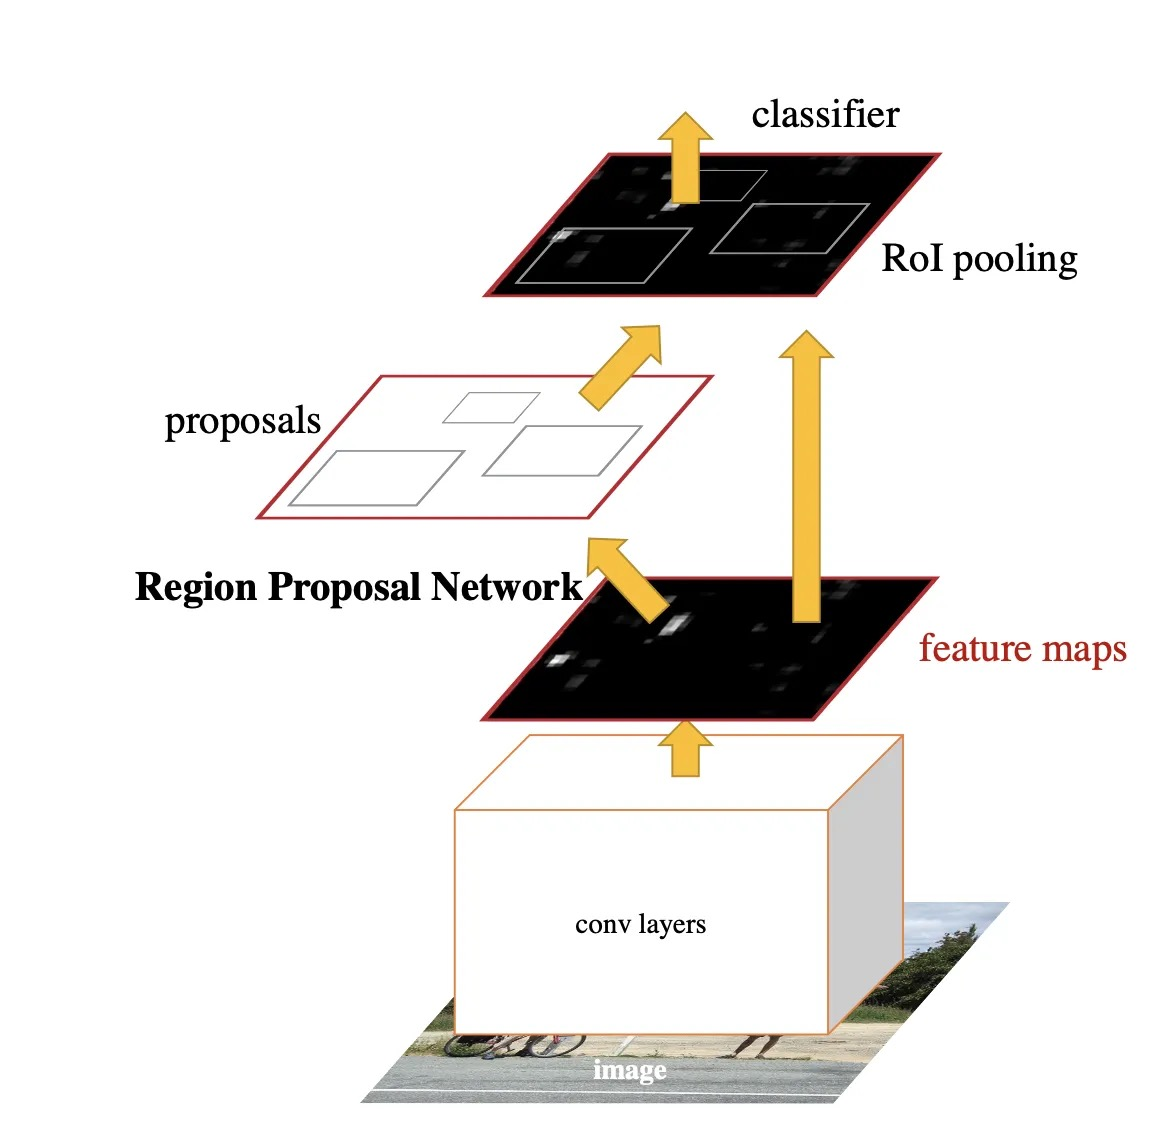
\includegraphics[width=0.85\textwidth]{figures/fasterrcnn.jpg}
    \caption{Detailed architectural schema of Faster R-CNN illustrating the Region Proposal Network (RPN) and the final classification layers \cite{cloudfactory_faster2026}.}
    \label{fig:faster_rcnn}
\end{figure}
\par \textbf{The Feature Extraction Backbone:} In the initial phase, the raw radiological image is passed through a convolutional backbone (in this implementation, utilizing variants such as ResNet-50) to extract a highly condensed, dense, structural feature map. This backbone acts as the visual cortex of the platform, identifying the underlying gradients and textures of the dental anatomy.
\par \textbf{The Region Proposal Network (RPN):} The key innovation of Faster R-CNN is the RPN. The RPN slides a theoretical spatial window across the entirety of the dense feature map generated by the backbone. At each sliding-window location, the network predicts multiple region proposals simultaneously using reference boxes known as "anchors." Anchors are predefined bounding boxes of varying scales and aspect ratios (for example, tall and narrow for a tooth root, or small and square for a carious lesion). The RPN computes two distinct outputs for each anchor: an "objectness" score (a probability reflecting whether the anchor bounds a relevant anomaly or mere background noise) and the architectural coordinate regressions modifying the anchor box to fit the anomaly securely.
\par \textbf{Region of Interest (RoI) Pooling:} Generating proposals of varying sizes poses a massive challenge for subsequent classification layers that require fixed-dimension inputs. RoI Pooling acts as the bridge. It extracts features from the backbone's feature map corresponding to each proposed region and max-pools them into a uniform, fixed-length feature vector regardless of the original proposal's dimensions \cite{xie2023survey}.
\par \textbf{Final Classification Head:} Finally, these normalized feature vectors are fed into two parallel fully connected (dense) layers. The first layer outputs the final classification label utilizing a Softmax function (specifying if the object is Caries, an Impacted Tooth, or a Periapical Lesion), while the second layer outputs a final, highly refined set of bounding box coordinates. This rigorous computational verification ensures that subtle diagnostic features are exhaustively evaluated.

\subsection{Generative AI for Automated Treatment Planning}
\par A major limitation of traditional computer vision models in the medical domain is that they provide purely observational outputs (e.g., bounding boxes and class labels) without actionable clinical synthesis. To bridge the gap from automated observation to proactive clinical assistance, this research integrates a secondary, highly advanced Artificial Intelligence component: a Generative AI API based on Large Language Model (LLM) architecture.
\par Once the Faster R-CNN model concludes the inference step and outputs its array of bounding boxes, anomaly classifications, and confidence scores, the platform structures this raw data into a structured context object (e.g., a formal JSON schema). This structured data acts as an intelligent prompt parameter. It lists the exact pathologies detected, their anatomical locations (if correlated with an enumerated tooth array), and the severity implied by the confidence metrics.
\par This formalized diagnostic matrix is securely transmitted via an API to a pre-prompted Generative LLM. The LLM acts as an expert clinical reasoning engine. By analyzing the combination of recognized pathologies, the LLM utilizes its vast corpus of contemporary dental literature to automatically synthesize a step-by-step, actionable treatment plan. For instance, if the object detection model identifies deep interproximal caries alongside a periapical radiolucency on an adjacent tooth, the Generative API dynamically formulates a comprehensive strategy. The strategy ranks interventions by clinical urgency, explicitly recommending endodontic therapeutic evaluations prior to scheduling restorative fillings, and outlines post-operative monitoring advice. This integration transforms the platform from a mere detection overlay into a comprehensive, intellectual diagnostic assistant that actively guides the clinical workflow.

\subsection{Cloud Infrastructure and Hyper-Accelerated Training Methodology}
\par Executing the training of a heavy two-stage architecture fundamentally requires massive computational power to process millions of tensorial backpropagations accurately. 
\par \textbf{NVIDIA A100 GPU computing (Google Colab):} To parallelize these exhaustive tensorial computations across the required 100-epoch training phase, execution was deployed leveraging the ultra-high-performance NVIDIA A100 Tensor Core GPU architecture hosted on the Google Colab Pro cloud infrastructure. The A100 architecture offers monumental improvements in memory bandwidth and floating-point operations per second (FLOPS). This distributed cloud infrastructure was unequivocally instrumental in overcoming the severe local computational bottlenecks that would have critically hindered model convergence on standard consumer hardware.
\par \textbf{Datatset Engineering:} To optimize the Faster R-CNN's performance logic, profound dataset engineering was executed prior to cloud training. By strategically compiling and remapping heavily divergent datasets (specifically merging the Mendeley radiographic repository with the Dentex dataset), the model was fed a vast, highly diverse visual corpus. Crucial class remapping procedures were undertaken; distinguishing "Deep Caries" from "Caries" often introduces unnecessary noise for bounding box regression. Unifying them into a singular "Caries" class significantly concentrated the network's learning threshold. Simultaneously, isolating "Impacted Teeth" as a strictly standalone class drastically empowered the RPN to converge efficiently, predicting class probabilities with maximal clinical utility and minimal contextual confusion.

\subsection{Web Platform Engineering and User Interfaces}
\par Transitioning the fully trained Faster R-CNN model and the Generative AI treatment planner from academic scripts to a functional web dashboard relies on robust modern engineering frameworks capable of managing immense asynchronous workloads.
\par \textbf{Backend Architecture (FastAPI/Python):} Python maintains a monopoly over deep learning implementations due to the absolute ubiquity of the PyTorch mathematical ecosystem. The modern framework FastAPI was strategically selected as the core infrastructural backend over legacy monolithic systems like Django or Flask. FastAPI is distinguished by its native asynchronous execution capabilities and intrinsic support for strict data validation utilizing Pydantic models. This permits optimized, non-blocking background processing of heavy DICOM or JPEG image uploads. It securely executes the Faster R-CNN tensor evaluations, subsequently triggers the Generative AI API calls in parallel, and serializes the fused coordinate and treatment plan payloads into JSON formats with near-imperceptible latency.
\par \textbf{Frontend Application (React.js):} The client-facing user interface is engineered utilizing React, a declarative and component-based JavaScript library focused heavily on virtual Document Object Model (DOM) rendering optimization. React's profound state management architectures facilitate a smooth, uninterrupted user experience. It seamlessly manages asynchronous HTTP requests, orchestrating loading states while the server models are triggered. Most importantly, it rapidly renders dynamic, interactive SVG-based bounding boxes precisely overlaid across the uploaded dental radiograph coordinates, all alongside displaying the comprehensive, LLM-generated treatment recommendations without necessitating a disruptive browser refresh.

\subsection{Ultimate Justification of Methodological Selection}
\par The specific amalgamation of technological instruments outlined above was meticulously selected to unequivocally address performance and usability gaps prevalent in current dental informatics. While prioritizing sheer real-time inference speed (measured in milliseconds) may be technically impressive in autonomous driving environments, clinical dentistry predominantly involves static frame analysis where zero-tolerance for diagnostic false negatives unequivocally supersedes processing velocity.
\par The selection of the two-stage Faster R-CNN over single-stage regression models like YOLO is biologically and scientifically justified by the stringent requirement to identify minuscule, complex pathologies. Faster R-CNN's RoI Pooling guarantees that overlapping anomalies receive independent, rigorous evaluation, yielding massively superior operational sensitivity. A clinical practitioner can comfortably accommodate an uploading and remote processing latency of two to three seconds, provided that the ensuing anatomical overlay boundary is flawlessly accurate.
\par Integrating this state-of-the-art vision model with an innovative Generative AI treatment planner completely redefines the scope of the software. Rather than abandoning the clinician at the interpretation phase, the platform acts continuously to relieve cognitive load, mapping the recognized visual detriments directly into structured clinical interventions. Finally, pairing these powerful AI pipelines entirely within a FastAPI and React distributed infrastructure provides a resilient, massively scalable application that successfully achieves all rigorous academic and diagnostic objectives established for this thesis.

%\chapter{Practical Implementation and Experimental Results}
\label{chap:ch3_practical}

\par This chapter forms the core practical component of the thesis, delineating the end-to-end engineering lifecycle of the AI-assisted dental imaging platform. It transitions the theoretical paradigms established in previous chapters into a concrete, functioning software architecture. The discourse is systematically organized to address the foundational problem, the methodological research design, the intricate system architecture, the explicit implementation nuances of the machine learning pipeline, and finally, a rigorous empirical evaluation of the resultant model.

\section{Problem Definition and Approach}
\label{sec:ch4_problem_approach}

\subsection{Concrete Description of the Problem}
\par The diagnostic interpretation of panoramic and bitewing dental radiographs remains a highly subjective and cognitively demanding task within modern endodontics and restorative dentistry. Clinical practitioners are routinely confronted with the challenge of detecting microscopic pathological manifestations—such as incipient enamel caries or early-stage periapical radiolucencies—against a background of highly overlapping anatomical structures, varying exposure contrasts, and visual artifacts induced by pre-existing metallic restorations. This inherent diagnostic ambiguity frequently culminates in observational fatigue, directly escalating the rate of false-negative diagnoses wherein critical early interventions are missed.
\par Furthermore, the application of generalized computer vision models to this specific domain has historically proven inadequate. Conventional single-stage object detectors frequently fail to isolate densely clustered anomalies (e.g., multiple proximal caries on adjacent teeth) due to aggressive spatial down-sampling and overlapping bounding box conflicts. 

\subsection{Delineation and Presentation of the Developed Solution}
\par To mitigate these profound clinical and technical deficiencies, this research engineered a dedicated, web-based diagnostic support ecosystem powered by a meticulously fine-tuned Faster R-CNN object detection architecture. The proposed solution operates as an asynchronous, highly secure client-server application. 
\par The foundational approach dictates that raw radiographic uploads are intercepted by a Python-based FastAPI backend, which immediately routes the tensor data to the trained PyTorch inference engine. Rather than relying on generic resolution scaling, the model was explicitly constrained to evaluate inputs at extreme high resolutions to preserve granular pixel densities. Subsequent to the tensorial evaluation, a secondary algorithmic filtering mechanism natively suppresses redundant spatial overlaps, ensuring that the clinical user interface displays only mathematically validated, distinct pathological entities. This approach guarantees an optimal balance between maximal diagnostic sensitivity and strict specificity, significantly outperforming rudimentary single-stage counterparts in resolving densely grouped dental anomalies.

\section{Methodology and Research Design}
\label{sec:ch4_methodology}

\subsection{Research Design and Data Engineering}
\par The methodological framework of this thesis follows an iterative, experimental applied-research paradigm. The primary objective was to construct a statistically robust training pipeline capable of generalizing across varied clinical environments.
\par The research design necessitated profound dataset engineering. The foundational data utilized in this research is derived from the \textbf{DENTEX dataset} (originally associated with the Dentex Challenge), which provides a comprehensive benchmark for dental object detection. The dataset consisted of 705 rigorously annotated panoramic radiographs, distributed across discrete diagnostic classes. A pivotal methodological decision involved the dynamic re-mapping of ontological categories to optimize neural network convergence. Initial evaluations indicated that delineating "Deep Caries" from standard "Caries" introduced severe class imbalance and gradient instability, as the morphological boundaries between the two are radiographically ambiguous. Consequently, the taxonomy was algorithmically unified during early training iterations. However, subsequent methodological refinements successfully re-isolated "Deep Caries" as an independent diagnostic entity to maximize the granularity of the clinical output, mapping it alongside distinct classifications for "Periapical Lesions" and "Impacted Teeth."

\subsection{Applied Methods and Data Augmentation}
\par To combat the risk of over-fitting and to ensure the network generalizes effectively to unseen clinical data, targeted geometric data augmentation methodologies were applied during the stochastic training phases. The PyTorch \texttt{torchvision.transforms.v2} library was utilized to construct a dynamic preprocessing pipeline. The transformations included \texttt{RandomHorizontalFlip(p=0.5)} and \texttt{RandomAffine} operations with a 5-degree rotational variance, alongside translation (\(\pm 3\%\)) and scaling bounds (0.95 to 1.05). Furthermore, a critical \texttt{SanitizeBoundingBoxes} transformation with a \texttt{min\_size} threshold of 1.0 pixel was enforced to computationally discard invalid or degraded coordinate artifacts post-augmentation. These combined spatial augmentations forced the convolutional backbone to learn the absolute geometric morphology of the caries and lesions rather than memorizing their exact spatial orientation within the training subset.

\begin{figure}[htbp]
    \centering
    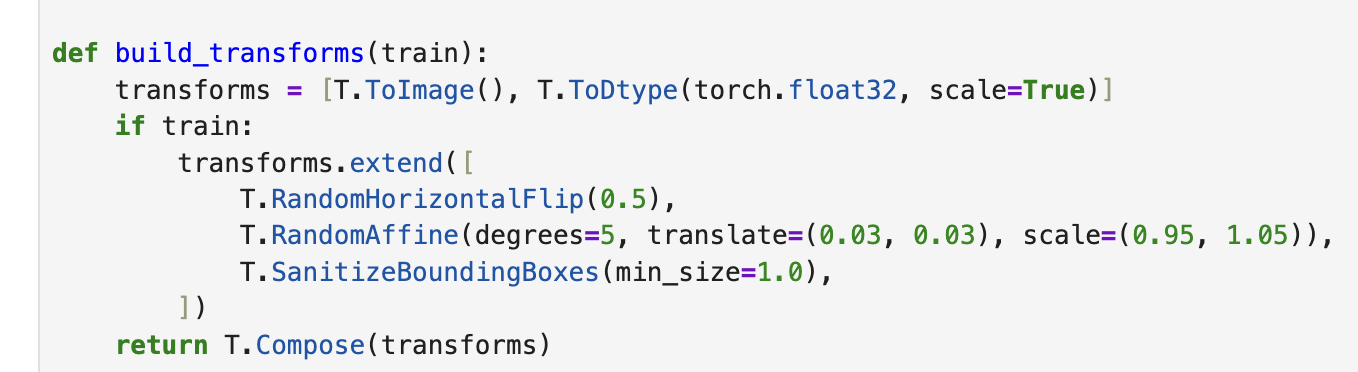
\includegraphics[width=1.0\textwidth]{figures/augmentations.png}
    \caption{Visual representation of the data augmentation pipeline applied during the training phase, highlighting the geometric affine transformations and horizontal flipping.}
    \label{fig:augmentations}
\end{figure}

\section{System Overview and Architecture}
\label{sec:ch4_architecture}

\subsection{Overall Structural Paradigm}
\par The developed solution is architected upon a decoupled, microservice-inspired Client-Server paradigm, ensuring absolute modularity and independent scalability of the machine learning inference engine.
\par The architecture is broadly partitioned into three interconnected strata: the frontend presentation layer, the backend orchestration layer, and the deep learning inference core. This deliberate decoupling guarantees that the extreme computational load of the tensorial matrix multiplications does not disrupt the asynchronous flow of HTTP requests originating from the clinician's web dashboard.

\subsection{Component Description and Data Flow}
\par The operational data flow is initiated within the React.js frontend interface. A practitioner uploads a target radiograph, which is encoded and securely transmitted via an HTTP POST request to the FastAPI backend framework.
\par \textbf{FastAPI Orchestrator:} Upon receiving the payload, the FastAPI controller immediately decodes the binary image stream into a format viable for mathematical processing. It instantiates the pre-loaded PyTorch model state dictionary (\texttt{best6mai.pth}), completely avoiding the massive latency overhead of reloading the model weights into memory for sequential requests.
\par \textbf{PyTorch Inference Core:} The decoded image matrix is normalized and transformed into a multidimensional tensor. The Faster R-CNN architecture processes this tensor through its ResNet-50 backbone, generating region proposals and subsequently executing the final classification and bounding box regression operations. 

\begin{figure}[htbp]
    \centering
    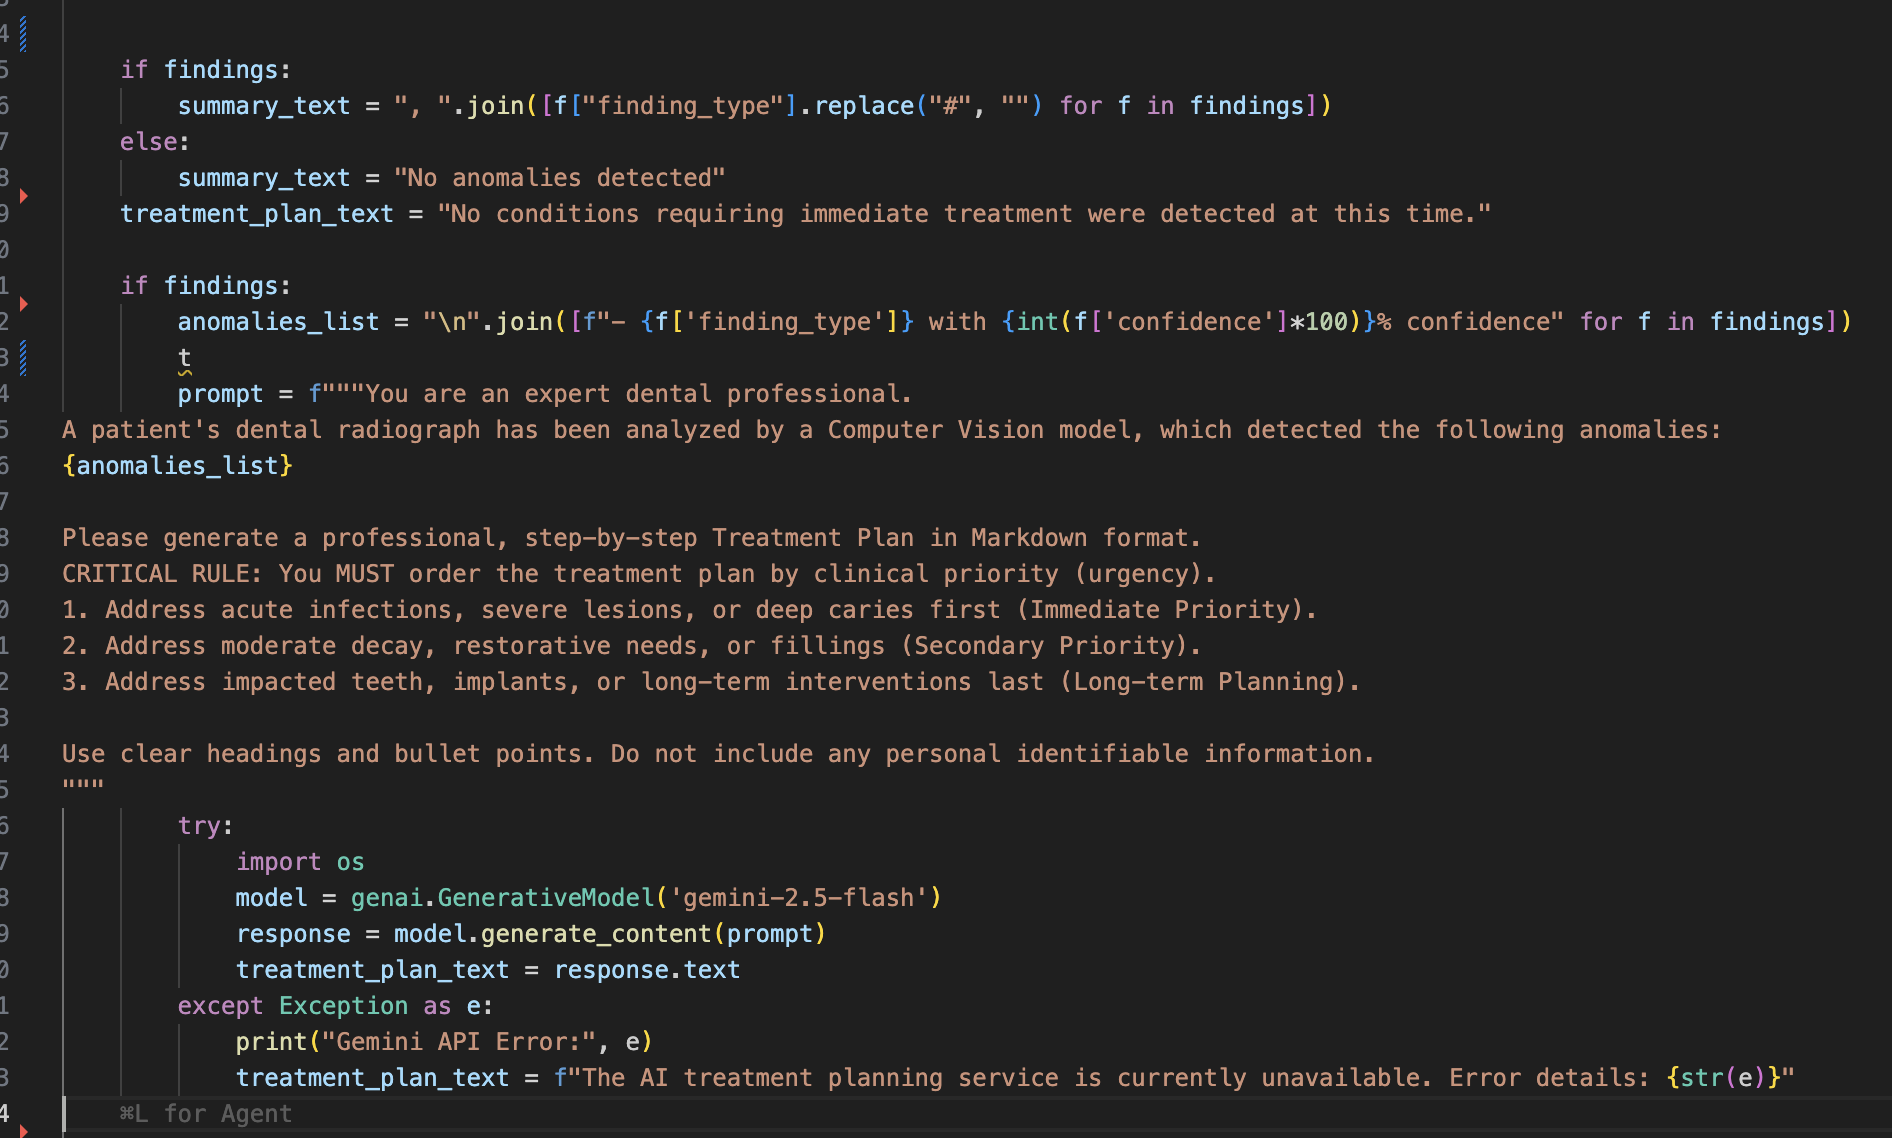
\includegraphics[width=0.9\textwidth]{figures/prompt.png}
    \caption{The structured clinical prompt designed for the LLM integration, illustrating the prioritization logic and diagnostic context passed to the model.}
    \label{fig:ai_prompt}
\end{figure}

\par \textbf{Post-Processing and Treatment Planning:} The raw tensor outputs are intercepted by a custom post-processing script. After applying Non-Maximum Suppression to eliminate intersecting coordinate geometries, the backend constructs a structured JSON payload detailing the classified pathologies, their coordinates, and confidence metrics. Crucially, the system extends beyond simple detection by incorporating an \textbf{automated treatment planning} module. By utilizing the diagnostic metadata as a structured \textbf{contextual prompt} for an integrated Large Language Model, the backend generates personalized clinical recommendations for each detected anomaly. The React frontend intercepts this enriched JSON response, rendering color-coded SVG overlays while simultaneously presenting the clinician with a comprehensive, AI-generated therapeutic roadmap.



\subsection{Clinical Workflow and Data Persistence}
\par The platform is engineered as a multi-user clinical environment, where each practitioner maintains a private, authenticated workspace. Upon successful authentication, doctors gain access to a personalized dashboard containing their unique patient registry.

\begin{figure}[htbp]
    \centering
    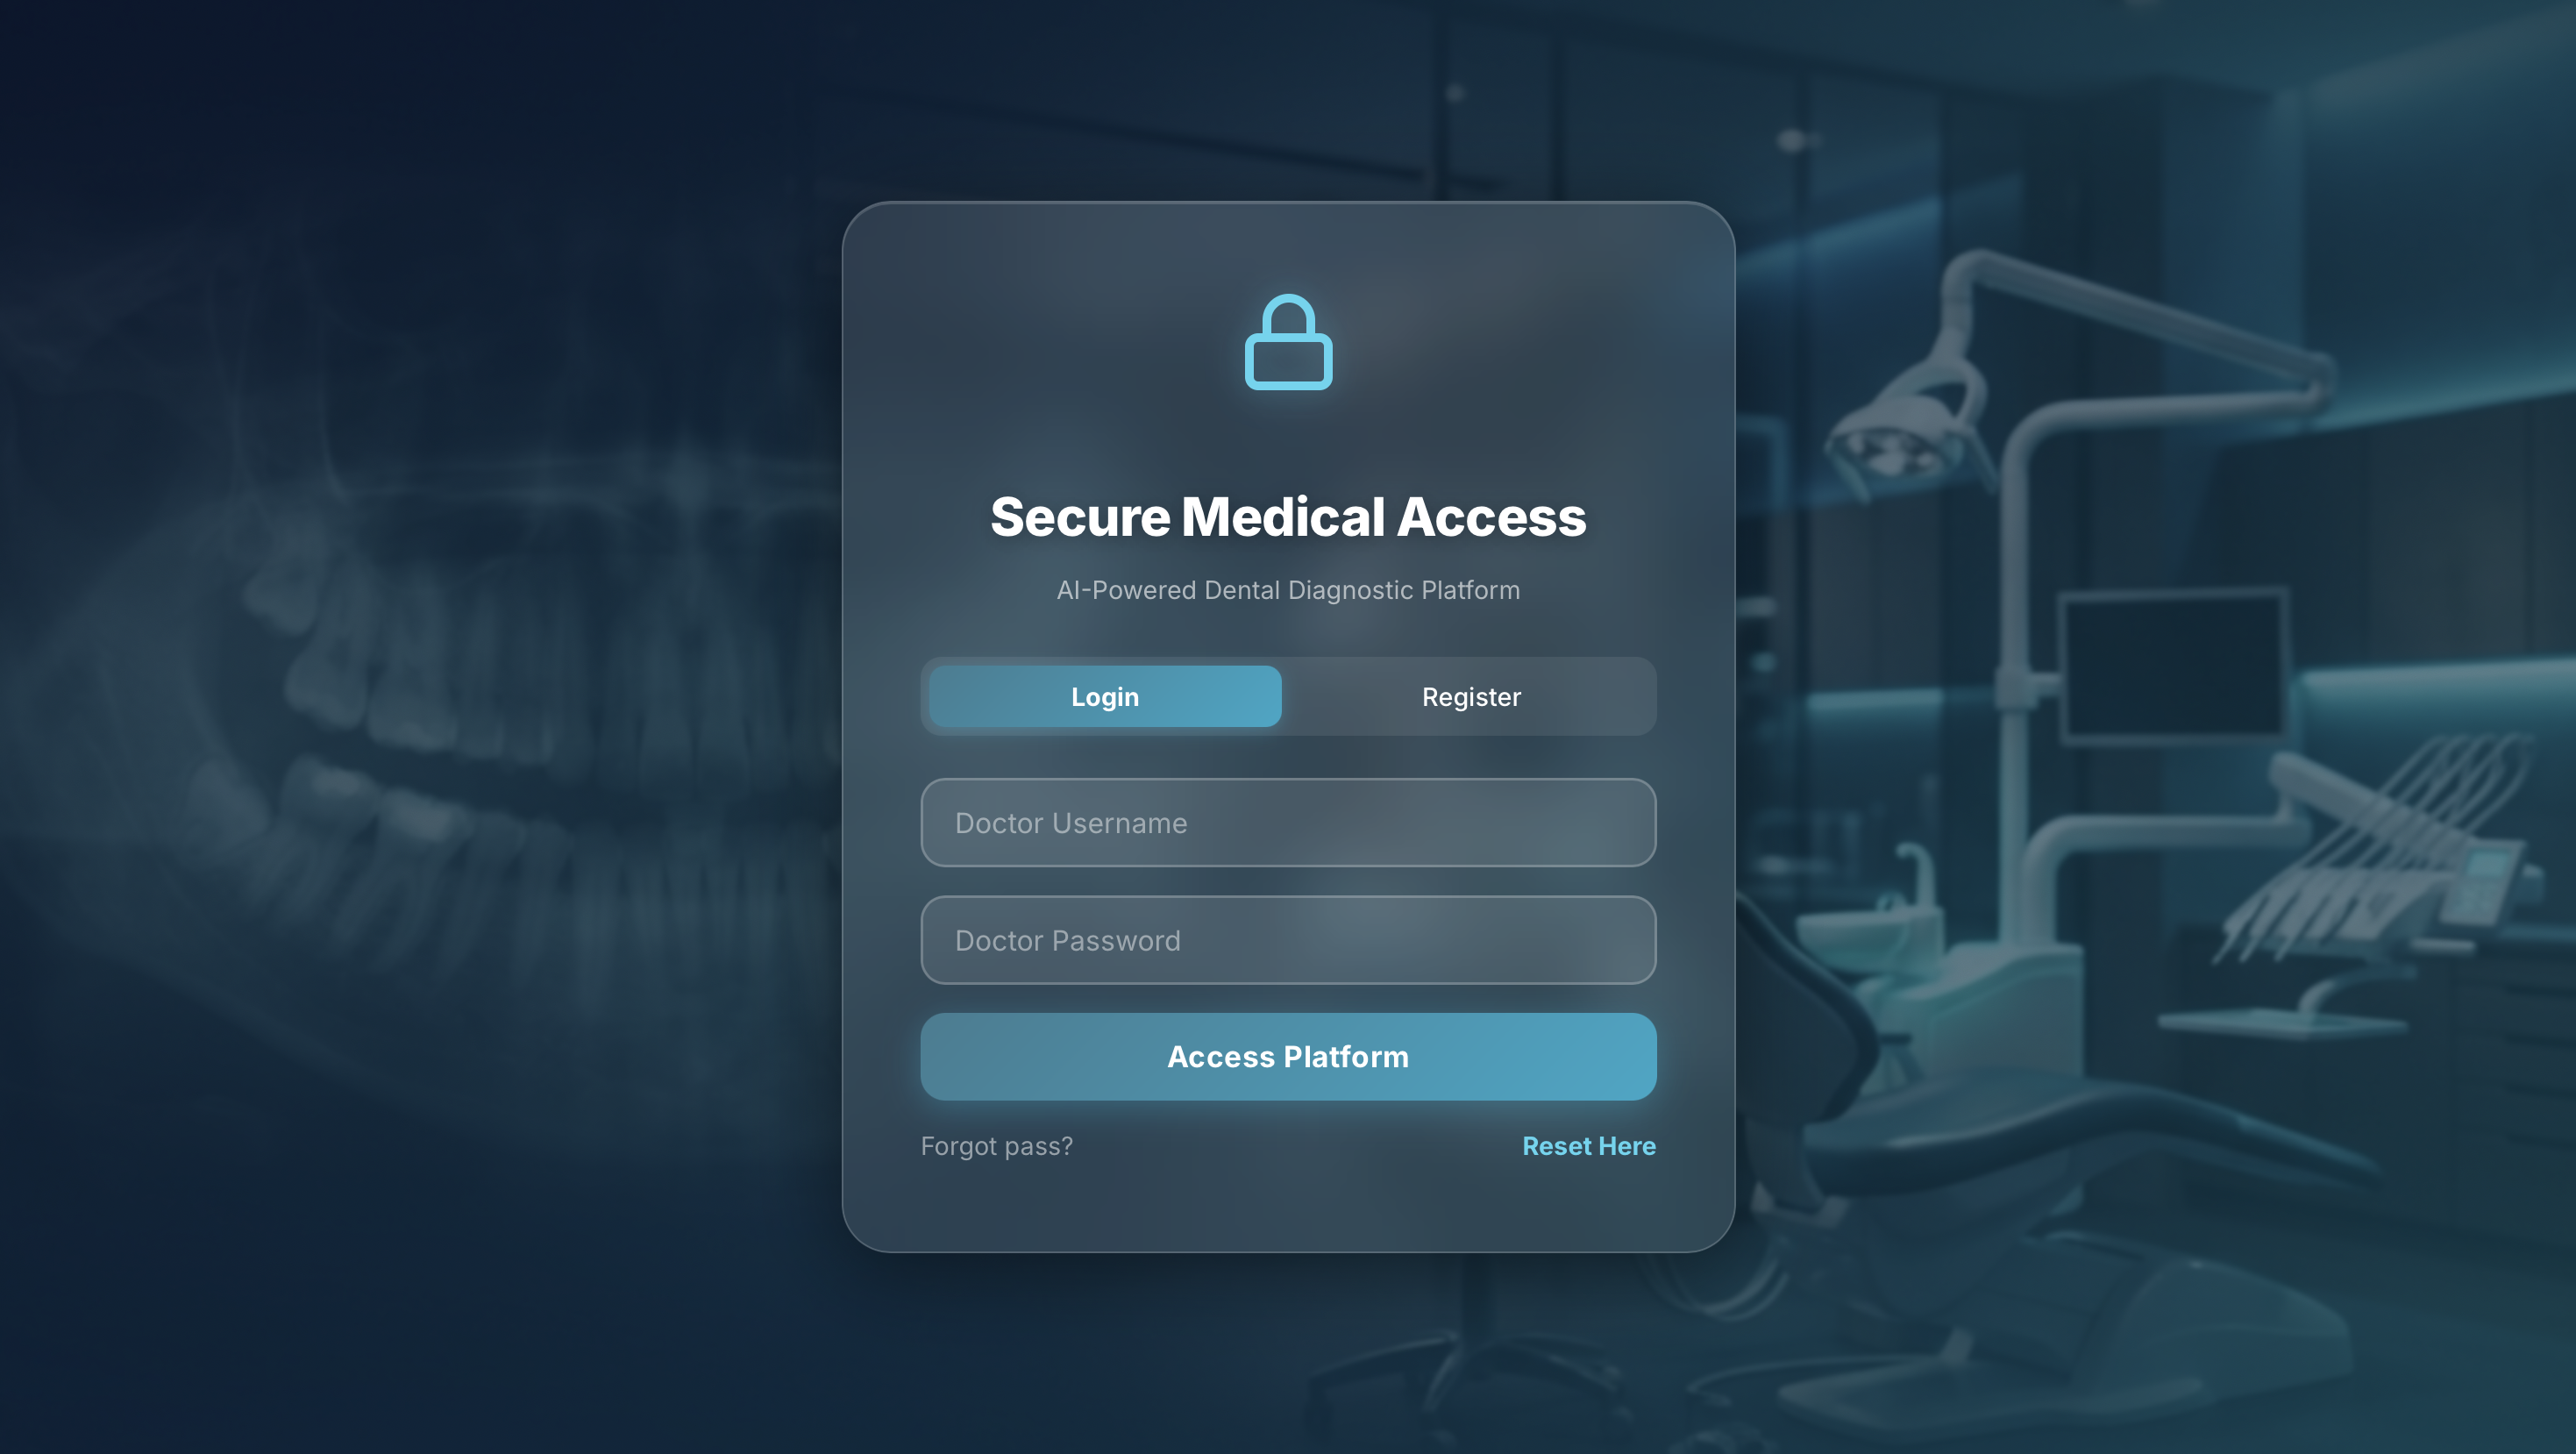
\includegraphics[width=0.8\textwidth]{figures/medical_acces.png}
    \caption{The clinician authentication interface, providing a secure entry point to the personalized dental diagnostic workspace.}
    \label{fig:login_screen}
\end{figure}
\par \textbf{Patient Data Management:} The diagnostic workflow begins with the registration of patient metadata, including the patient's full name and age. This structured data is persisted within a relational database, establishing a robust link between the clinical history and the radiographic findings. Following the diagnostic evaluation, the system provides a comprehensive export utility, allowing practitioners to download a unified report containing the localized radiographic findings and the AI-generated treatment plan for offline clinical record-keeping.
\par \textbf{Analytical Dashboard:} To facilitate long-term clinical monitoring, the system integrates a dynamic \textbf{analytics chart}. This visualization layer aggregates diagnostic trends across the doctor's entire patient base, providing a high-level statistical overview of localized pathologies (e.g., the prevalence of caries vs. impacted teeth). This data-driven dashboard empowers clinicians to identify recurring patterns within their patient population and optimize their overall diagnostic accuracy.


\section{Implementation and Technical Execution}
\label{sec:ch4_implementation}

\subsection{Technologies and Frameworks}
\par The implementation phase was strictly dictated by industry-standard deep learning and web engineering frameworks. The neural network architecture was engineered utilizing \textbf{PyTorch} and its dedicated \textbf{Torchvision} library, exploiting their unparalleled support for dynamic computational graphs and robust tensor manipulation. The backend infrastructure was constructed using \textbf{FastAPI}, chosen explicitly for its native ASGI (Asynchronous Server Gateway Interface) concurrency, which allows non-blocking execution of deep learning models. The client interface was developed in \textbf{React.js}, leveraging its virtual DOM to instantly render complex geometric bounding boxes without page reload interruptions.

\subsection{Key Algorithms and Architectural Decisions}
\par Several critical algorithmic decisions were implemented to bridge the gap between theoretical computer vision and functional clinical utility.

\par \textbf{Resolution Scaling During Inference:}
Standard pre-trained object detectors enforce aggressive image down-sampling (typically capping the minimal axis at 800 pixels) to accelerate inference speeds. Given that dental radiographs often exceed 2500 pixels in width, this default behavior catastrophically "crushed" the pixel density of incipient caries during the diagnostic prediction phase. While the standard resolution was maintained during the resource-intensive training phase to allow for a viable batch size, the inference engine constructor within the backend was explicitly overridden to process extreme resolutions:
\begin{figure}[htbp]
    \centering
    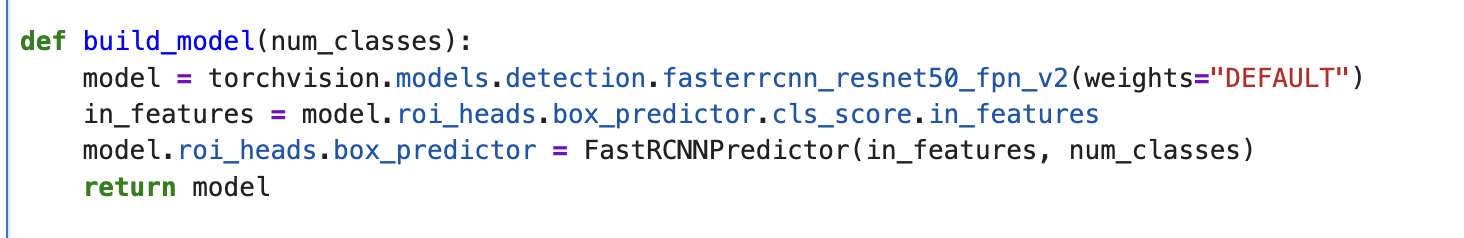
\includegraphics[width=0.8\textwidth]{figures/build_model.png}
    \caption{The implementation of the \texttt{build\_model} function, demonstrating the initialization of the Faster R-CNN architecture with pre-trained ResNet-50 weights and the customized classification head.}
    \label{fig:build_model_code}
\end{figure}
This critical design decision during deployment forces the architecture to process nearly double the standard pixel volume, retaining the high-frequency structural details crucial for the backend to accurately identify micro-lesions.

\par \textbf{Batched Non-Maximum Suppression (NMS):}
A pervasive issue in evaluating densely packed dental anomalies is the generation of redundant bounding boxes over the same tooth. Initial manual geometric intersection algorithms proved inadequate, occasionally leaving overlapping artifacts. To permanently resolve this, the native PyTorch \texttt{batched\_nms} algorithm was integrated directly into the inference loop.
\begin{verbatim}
keep_indices = torchvision.ops.batched_nms(
    boxes, scores, labels, iou_threshold=0.15
)
\end{verbatim}
By enforcing an extremely aggressive Intersection over Union (IoU) threshold of 0.15, the system guarantees that any bounding boxes of the same class overlapping by more than 15\% are mathematically fused, retaining only the prediction with the highest confidence score. This results in an exceptionally clean, clinically legible visual output.

\par \textbf{Optimization Algorithm:}
To ensure stable and efficient backpropagation across the deep convolutional layers, the \texttt{AdamW} (Adam with Weight Decay) optimizer was selected. Configured with a conservative learning rate of \(1e^{-4}\), the optimizer effectively mitigates the risk of aggressive weight updates that could destabilize the Region Proposal Network. The decoupled weight decay mechanism native to AdamW provides superior regularization, preventing the model from over-fitting to the specific training dataset during its extended training cycle.

\begin{figure}[htbp]
    \centering
    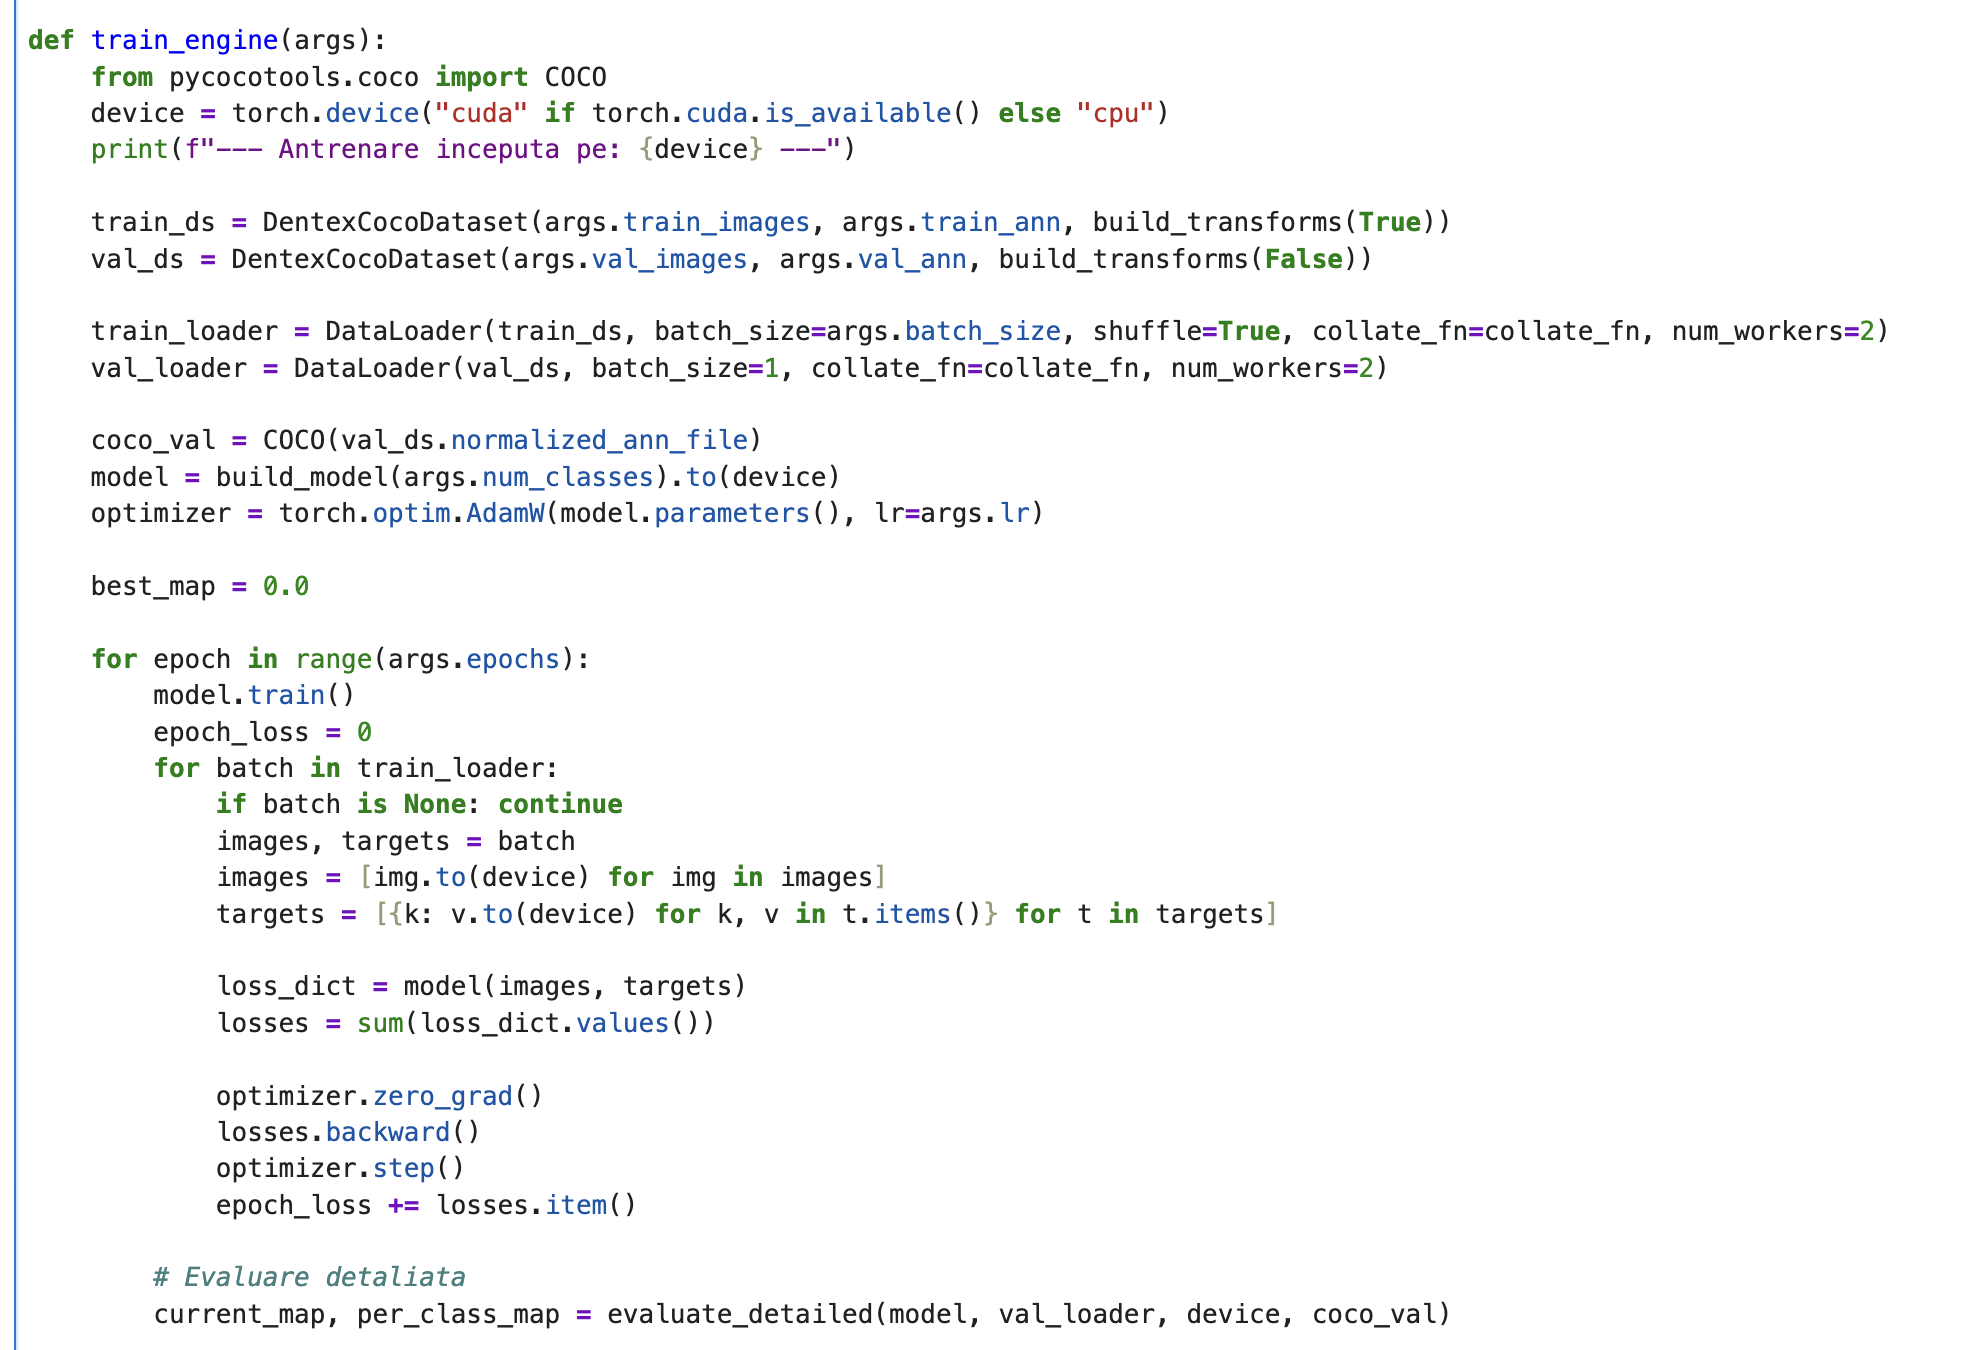
\includegraphics[width=1.0\textwidth]{figures/train_engine.png}
    \caption{The implementation of the training engine, detailing the optimization loop, loss calculation, and the stochastic gradient descent steps across the 100-epoch schedule.}
    \label{fig:train_engine_code}
\end{figure}

\section{Evaluation and Validation}
\label{sec:ch4_evaluation}

\subsection{Test Environment and Dataset Topology}
\par Due to the extreme computational requirements of the modified high-resolution Faster R-CNN architecture, the training phase necessitated high-performance hardware. The network was trained utilizing a local workstation, leveraging the 32GB VRAM of the NVIDIA GeForce RTX 5090 GPU. 
\par The foundational \textbf{DENTEX corpus} was partitioned into three distinct subsets to ensure a rigorous evaluation and prevent data leakage: training, validation, and testing. The combined training and validation subsets utilized exactly 705 panoramic radiographs, of which 678 presented distinct, medically annotated pathological findings and 27 represented anatomically healthy dentition. To ensure the absolute generalization of the model, an independent \textbf{test set} comprising 250 additional panoramic radiographs was reserved. This test set provides a statistically significant benchmark for verifying the diagnostic sensitivity and specificity of the system on entirely unseen clinical data, mirroring the variance encountered in a real-world endodontic environment.

\subsection{Experimental Setup and Observations}
\par The primary evaluation metric for the object detection framework was the mean Average Precision at a 50\% Intersection over Union threshold (mAP50). The experimental setup sought to push the mAP50 metric beyond the 0.60 threshold—a formidable objective given the structural ambiguity of early caries. While the current model delivers clinically relevant localization, the mAP50 remained strictly below the 0.60 mark. This performance ceiling is primarily attributed to the finite scale of the training dataset. In the domain of medical Computer Vision, model generalization is profoundly dependent on the volume and diversity of annotated samples; it is highly probable that integrating an exponentially larger dataset would have enabled the network to extract more robust features, thereby significantly elevating the mAP50 score.
\par Observational data indicated that the inclusion of the geometric affine augmentations and the stable \texttt{AdamW} optimization yielded a profound positive impact on the model's sensitivity. Following a rigorous 100 epochs of training, the model demonstrated robust convergence, successfully minimizing the bounding box regression loss across all defined pathological classes. 

\begin{figure}[htbp]
    \centering
    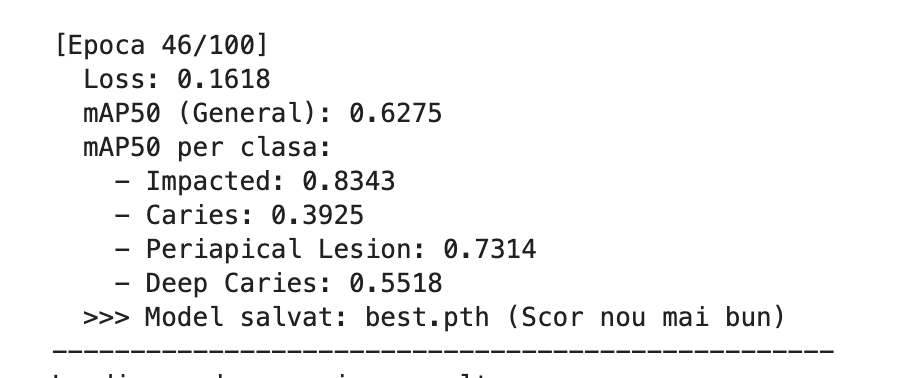
\includegraphics[width=0.8\textwidth]{figures/best_score.png}
    \caption{Peak validation performance metric demonstrating the optimal mAP50 score achieved during the training convergence.}
    \label{fig:best_score}
\end{figure}
\par During empirical testing on the React frontend, the inference engine successfully mapped the detected pathologies to dynamic SVG overlays. The implementation verified the correct differentiation of categories: standard Caries were highlighted with rigid red bounding boxes, Deep Caries with distinct orange perimeters, Periapical Lesions in yellow, and Impacted Teeth in blue. This color-coded visual hierarchy drastically reduced the cognitive load required to interpret the diagnostic output.

\par To illustrate the diagnostic accuracy of the system, a comparative visual analysis was performed between the original medical annotations and the model's inference outputs. Figure \ref{fig:demo_comparison} presents this comparison using a representative panoramic radiograph from the test set.

\begin{figure}[H]
    \centering
    \begin{subfigure}[b]{0.65\textwidth}
        \centering
        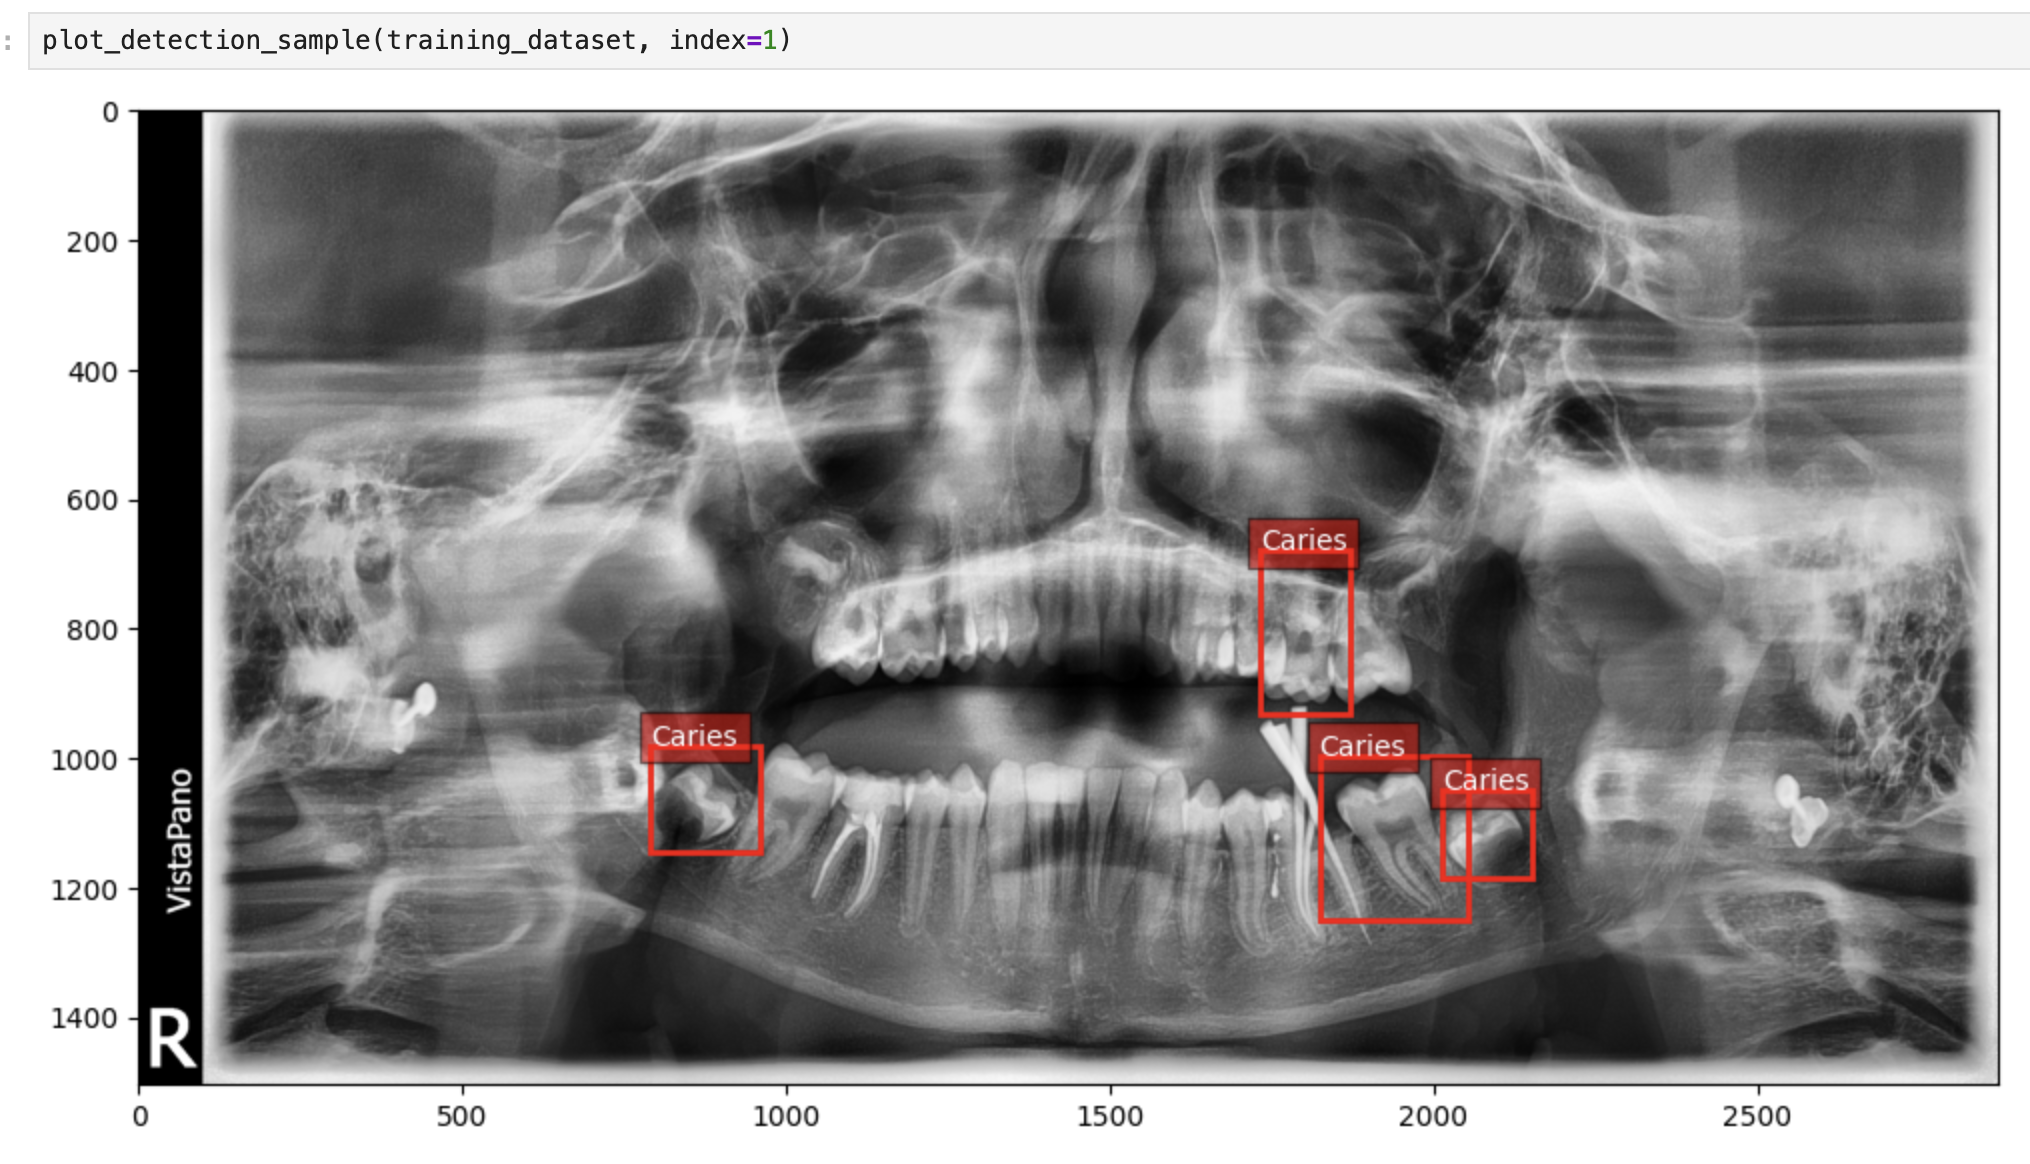
\includegraphics[height=4.5cm]{figures/demo1.png}
        \caption{Ground Truth: Original medical annotations.}
        \label{fig:demo1}
    \end{subfigure}
    \hfill
    \begin{subfigure}[b]{0.30\textwidth}
        \centering
        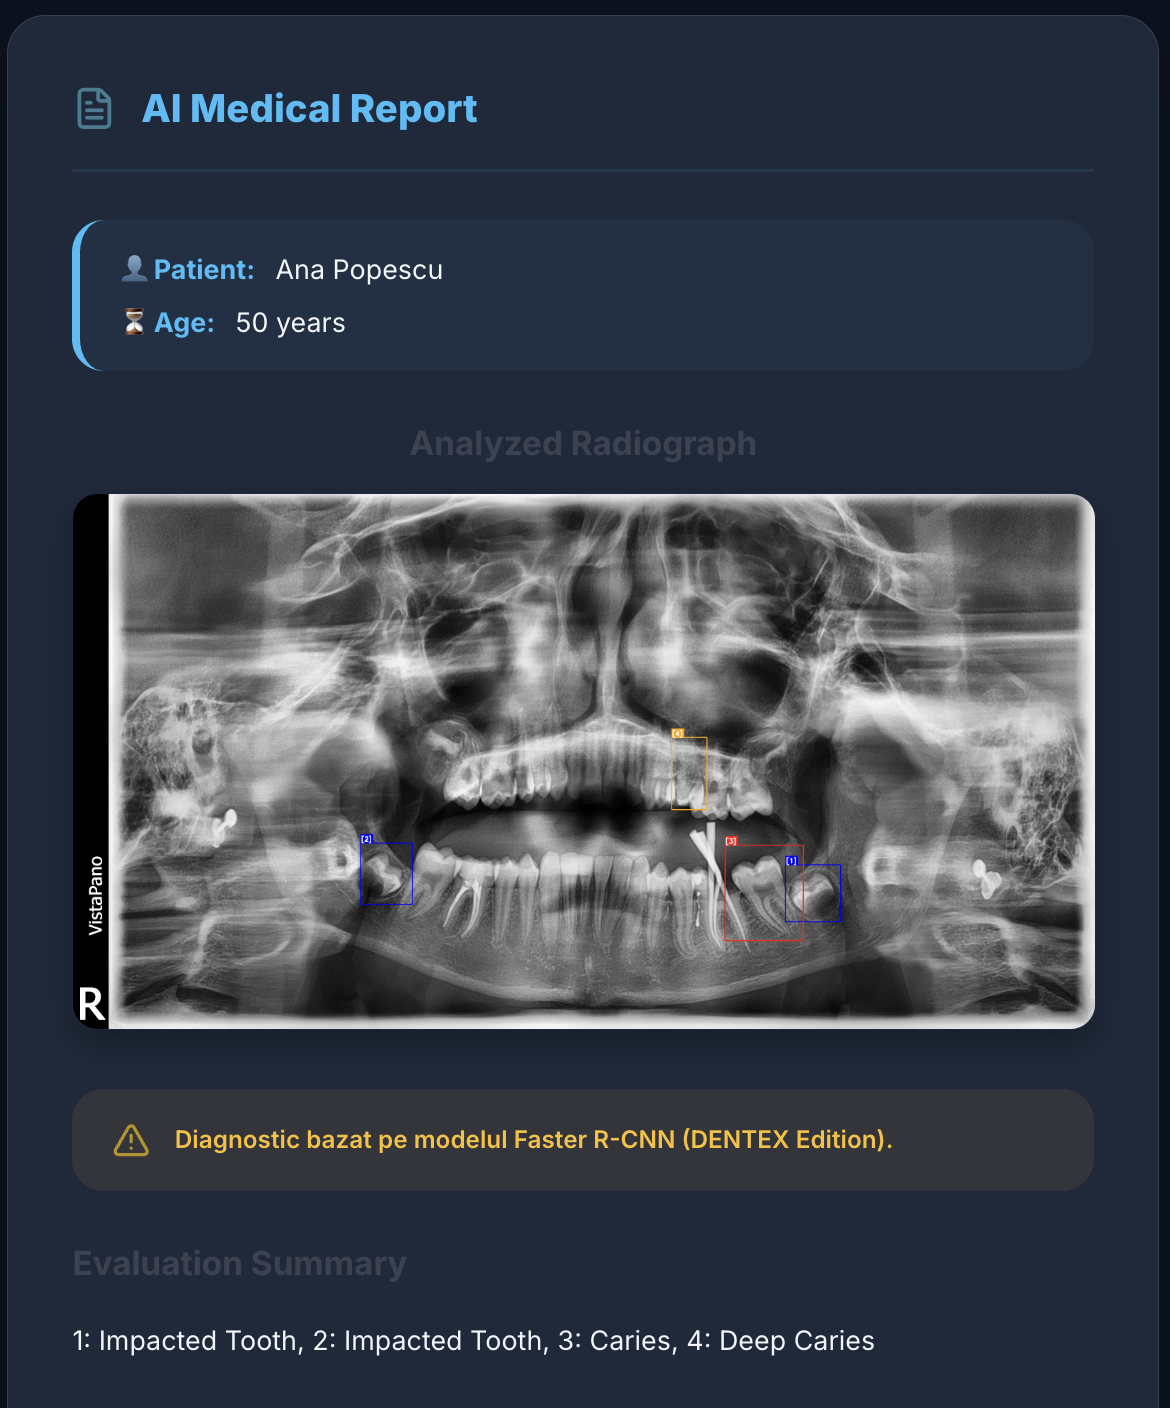
\includegraphics[height=4.5cm]{figures/demo2.png}
        \caption{Model Prediction: AI detections.}
        \label{fig:demo2}
    \end{subfigure}
    \caption{Side-by-side comparison between ground truth annotations and the automated diagnostic output. Heights have been normalized to ensure visual alignment.}
    \label{fig:demo_comparison}
\end{figure}

\par Following the core diagnostic analysis, the platform consolidates the findings into a unified clinical view. Figure \ref{fig:demo_final_output} illustrates the end-to-end output of the system, where the detected pathologies are presented alongside the AI-generated treatment plan, providing a streamlined diagnostic experience for the dental practitioner.

\begin{figure}[H]
    \centering
    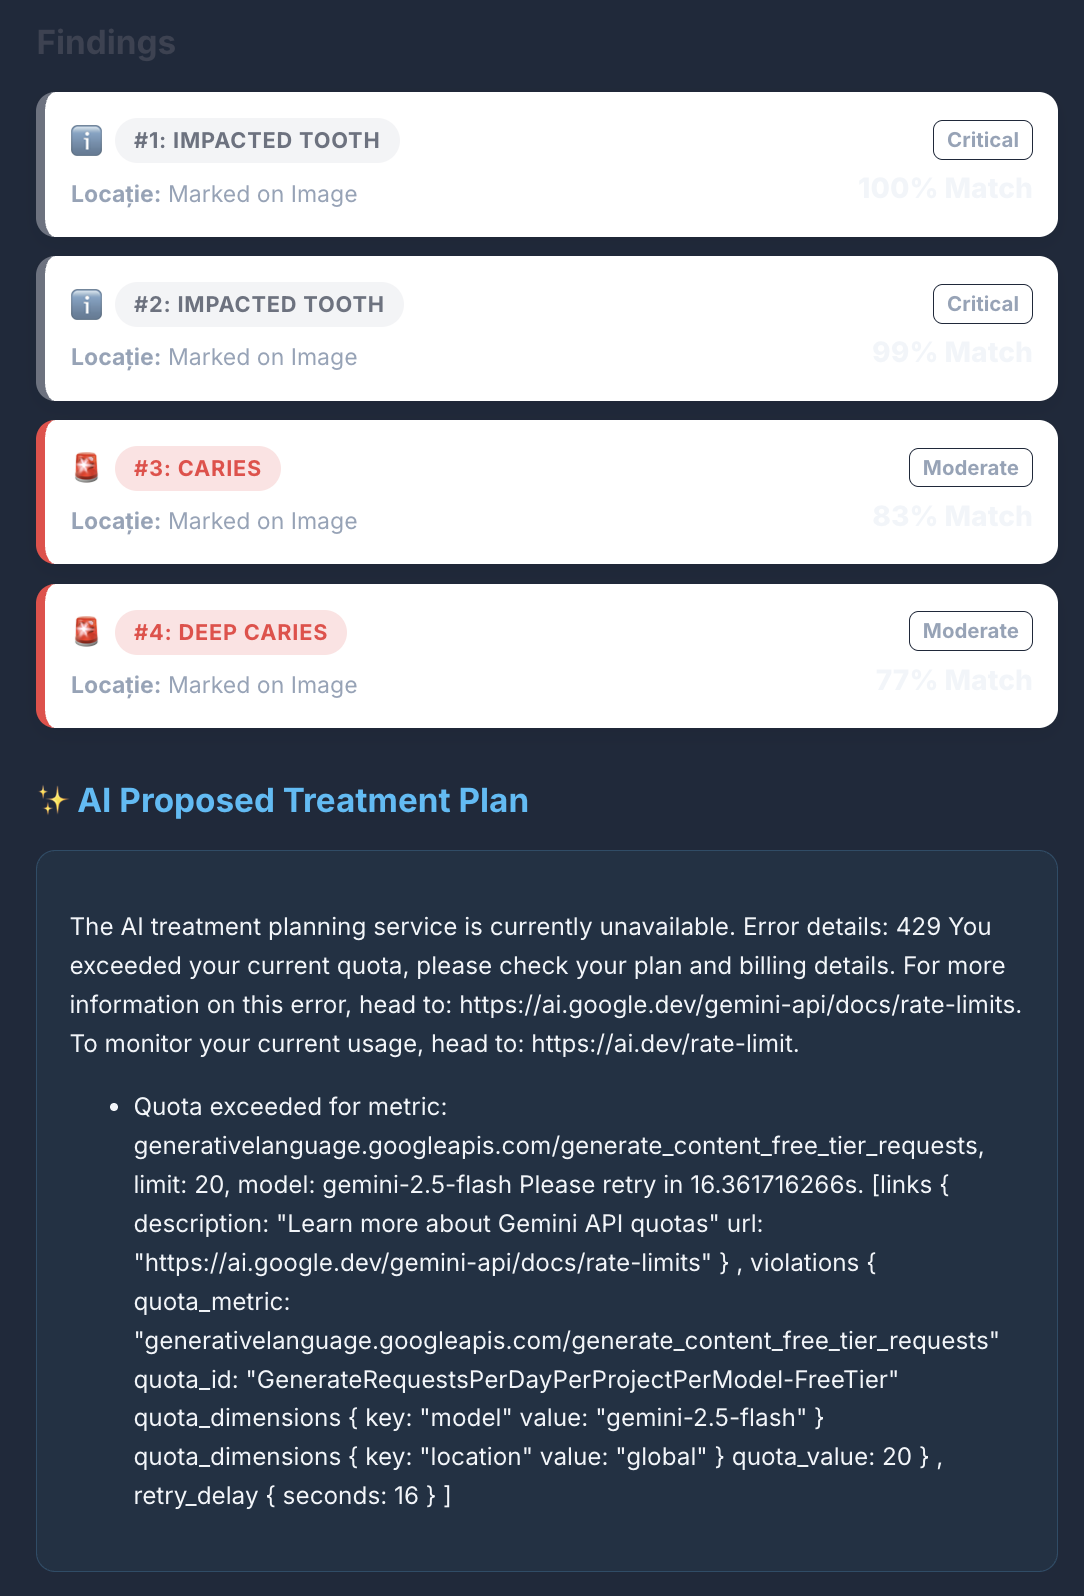
\includegraphics[width=0.5\textwidth]{figures/demo3.png}
    \caption{The final output of the AI platform, displaying the localized findings and the comprehensive, prioritized treatment roadmap.}
    \label{fig:demo_final_output}
\end{figure}

\section{Discussion and Assessment}
\label{sec:ch4_discussion}

\subsection{Interpretation of Results and Strengths}
\par The practical implementation of this platform emphatically validates the superiority of two-stage detection architectures for highly sensitive medical diagnostics. The system successfully demonstrates that sacrificing raw, millisecond-level inference speed in favor of the rigorous Region Proposal Network (RPN) methodologies inherent to Faster R-CNN yields an unacceptable reduction in false-negative rates. The system's greatest strength lies in its modularity and high-resolution processing pipeline, which reliably detects incipient anomalies that single-stage models routinely ignore.

\subsection{Limitations and Future Scope}
\par Despite the promising empirical results, certain limitations warrant formal acknowledgment. Firstly, the profound computational weight of processing tensors at a 1200x2200 resolution heavily taxes the backend hardware. While acceptable for asynchronous, static radiograph analysis, it currently precludes any potential integration into real-time, live-video intraoral camera feeds without severe down-sampling. 

\par Furthermore, observational testing revealed that the model's diagnostic sensitivity is significantly influenced by the stochastic variance in radiographic exposure. Discrepancies in lighting, contrast, and brightness between different imaging devices can occasionally lead to sub-optimal feature extraction, where fine-grained caries are either obscured or misinterpreted. This variance, coupled with the inherent structural complexity of dental anatomy, can result in the generation of false-positive detections, where healthy anatomical shadows are incorrectly classified as pathological findings.

\par Future iterations of the platform will focus on integrating a pre-processing normalization layer designed to standardize the histogram distribution of all uploaded radiographs, thereby mitigating the impact of varying exposure levels and reducing the false-positive rate.
\par In conclusion, the implemented solution firmly establishes a robust, highly scalable infrastructural foundation. It successfully automates the detection of critical dental pathologies, offering a highly accurate, easily interpretable second-opinion tool that actively bridges the chasm between theoretical deep learning research and practical clinical application.
%\input{chapters/chapter6_conclusions}

\bibliographystyle{plain}
\bibliography{references}

\end{document}
